\chapter{PREDICTIVE MODELING AND SURROGATE RISK ESTIMATION}

\section{Dataset Profiling and Preprocessing}
The empirical foundation of CivicTwin rests upon a comprehensive dataset of 13,998 drainage conduit segments compiled for the Vellore City Municipal Corporation (CMC). The raw dataset was curated by integrating OpenStreetMap (OSM) highway and waterway vector ways with field municipal engineering survey logs and topographic DEM rasters.

Table~\ref{tab:dataset_features} details the primary features present in the preprocessed dataset, along with their physical units and statistical distributions across the municipal study area.

\begin{table}[h!]
\centering
\caption{Dataset Feature Profiles for CMC Drainage Conduits ($N = 13{,}998$)}
\label{tab:dataset_features}
\fontsize{9pt}{11pt}\selectfont
\begin{tabular}{|l|c|c|c|c|p{4.0cm}|}
\hline
\textbf{Feature Name} & \textbf{Type} & \textbf{Min} & \textbf{Median} & \textbf{Max} & \textbf{Description} \\
\hline
\texttt{segment\_id} & String & --- & --- & --- & Unique conduit identifier (OSM way ID) \\
\texttt{ward\_number} & Integer & 1 & 28 & 60 & Administrative municipal zone / cluster \\
\texttt{drain\_type} & Categorical & --- & --- & --- & Structural class (Open Concrete, Pipe, etc.) \\
\texttt{width\_m} & Continuous & 0.40 & 1.20 & 4.50 & Channel surface width (meters) \\
\texttt{depth\_m} & Continuous & 0.30 & 1.00 & 3.20 & Invert-to-crest channel depth (meters) \\
\texttt{elevation\_m} & Continuous & 142.1 & 186.4 & 265.8 & Ground invert elevation above MSL (meters) \\
\texttt{slope\_pct} & Continuous & 0.05 & 0.45 & 5.80 & Longitudinal hydraulic bed slope (\%) \\
\texttt{topographic\_wetness\_index} & Continuous & 4.20 & 8.75 & 18.40 & Beven-Kirkby wetness index ($\ln(a / \tan \beta)$) \\
\texttt{design\_capacity\_m3s} & Continuous & 0.05 & 0.98 & 12.50 & Unobstructed hydraulic design capacity \\
\texttt{runoff\_coefficient} & Continuous & 0.30 & 0.72 & 0.92 & Imperviousness surface runoff coefficient \\
\texttt{waste\_silt\_buildup\_pct} & Continuous & 0.0 & 48.5 & 95.0 & Surveyed sediment and silt blockage (\%) \\
\texttt{blockage\_risk\_level} & Discrete & 0 & 1 & 2 & Structural risk target (0: Low, 1: High, 2: Crit) \\
\hline
\end{tabular}
\end{table}

Data hygiene and preprocessing procedures included:
\begin{itemize}
    \item \textbf{Deduplication and Identifier Integrity:} Segment IDs were verified for uniqueness; duplicate records were discarded to maintain topological 1-to-1 node mappings.
    \item \textbf{Unit Normalization:} Inspection of surveyed silt values revealed whether records were encoded as fractional decimals ($[0.0, 1.0]$) or percentages ($[0.0, 100.0]$); all records were normalized to a uniform percentage scale $[0, 100]$.
    \item \textbf{Imputation of Missing Morphometric Values:} For conduit segments with missing elevation records, median elevation values grouped by spatial zone were imputed. Conduit cross-sectional areas with unrecorded dimensions were populated using median engineering defaults conditioned on conduit classification type.
    \item \textbf{Spatial Geometry Verification:} Polylines were verified against valid geographic coordinate bounding boxes ($12.85^\circ \le \text{lat} \le 12.98^\circ$, $79.05^\circ \le \text{lon} \le 79.22^\circ$). 37 conduits lacking geospatial coordinates were tagged as unmapped and excluded from active map dispatch.
\end{itemize}

\section{Feature Engineering and Hydromorphometric Indices}
To capture both structural channel properties and macro-topographic terrain dynamics, specialized hydromorphometric indices were synthesized:
\begin{enumerate}
    \item \textbf{Topographic Wetness Index (TWI):} Formulated by Beven and Kirkby \cite{beven1979physically}, the TWI measures the steady-state propensity of a landscape position to accumulate subsurface and surface moisture:
    \begin{equation}
    \text{TWI} = \ln\left(\frac{a}{\tan \beta}\right)
    \label{eqn:twi_formula}
    \end{equation}
    where $a$ represents the specific catchment contributing area per unit contour length ($\text{m}^2/\text{m}$) and $\beta$ is the local hydraulic slope gradient in radians. Conduits located in topographic depressions with high upstream drainage area exhibit high TWI values ($\text{TWI} > 12.0$), indicating natural pooling zones vulnerable to acute inundation.
    \item \textbf{Hydraulic Cross-Section Aspect Ratio:} The ratio of channel width to channel depth:
    \begin{equation}
    AR = \frac{\text{width\_m}}{\text{depth\_m}}
    \label{eqn:aspect_ratio}
    \end{equation}
    Shallow, wide channels ($AR > 3.0$) experience lower hydraulic radii and slower flow velocities under partial flow, accelerating solid sediment settling compared to deep, narrow masonry trenches.
    \item \textbf{Catchment Tributary Area Inversion:} Inverted from baseline peak runoff and storm intensity according to Eqn.~\ref{eqn:area_inversion}, bounding the effective contributing drainage basin for rational runoff calculation.
\end{enumerate}

\section{Spatial Clustering and Ward Demarcation}
Administrative boundaries within municipal corporations are frequently re-drawn, while informal drainage paths cross ward limits. To provide robust spatial grouping for municipal crew allocation, CivicTwin executes unsupervised $k$-means spatial clustering ($k = 60$) over conduit geographic centroids $(\bar{\phi}_v, \bar{\lambda}_v)$:
\begin{equation}
\min_{\mu_1, \dots, \mu_k} \sum_{j=1}^{60} \sum_{v \in C_j} \|\mathbf{x}_v - \mu_j\|^2
\label{eqn:kmeans_clustering}
\end{equation}
where $\mathbf{x}_v = (\bar{\phi}_v, \bar{\lambda}_v)$ is the centroid coordinate vector of conduit $v$ and $\mu_j$ represents the spatial cluster center. 

This spatial partitioning yields 60 contiguous operational zones (Zone 1 to Zone 60), ensuring that municipal supervisors can filter dispatch queues by compact geographic sectors, reducing crew transit travel time between consecutive desilting assignments.

\section{Random Forest Surrogate Formulation}
To evaluate baseline structural conduit vulnerability independently of real-time precipitation inputs, an ensemble Random Forest classifier is trained to predict the structural risk label \texttt{blockage\_risk\_level} $\in \{0, 1, 2\}$ \cite{breiman2001random}.

The feature vector $\mathbf{x}_i \in \mathbb{R}^{d}$ for conduit $i$ comprises:
\begin{equation}
\mathbf{x}_i = \big[\text{ward}, Q_{\text{design}}, \text{width}, \text{depth}, \text{elevation}, \text{slope}, \text{TWI}, i_{\text{rain}}, t_{\text{dur}}, C_{\text{runoff}}, S_{\text{silt}}, \mathbf{d}_{\text{type}}\big]
\end{equation}
where $\mathbf{d}_{\text{type}}$ denotes one-hot encoded indicator variables representing conduit construction typology (Open Concrete, Covered Masonry, Pipe Culvert, Natural Earthen Ditch).

The Random Forest constructs an ensemble of $B = 100$ decorrelated decision trees $\{T_b\}_{b=1}^B$. At each node split, a random subset of $m = \lfloor\sqrt{d}\rfloor$ features is evaluated to select the feature and threshold that maximizes the reduction in Gini impurity $\Delta I_G$:
\begin{equation}
I_G(p) = 1 - \sum_{c=0}^2 p_c^2
\label{eqn:gini_impurity}
\end{equation}
where $p_c$ is the proportion of class $c$ training samples at the node. 

To address class imbalance across risk categories (where severe critical blockages represent a minority class in field surveys), cost-sensitive balanced class weighting is applied:
\begin{equation}
w_c = \frac{N}{3 \cdot N_c}
\label{eqn:class_weights}
\end{equation}
where $N$ is the total number of training samples and $N_c$ is the frequency of class $c$. The final ensemble prediction for an unseen conduit $\mathbf{x}^*$ is determined via majority vote across all $B$ decision trees:
\begin{equation}
\hat{y} = \arg\max_{c \in \{0, 1, 2\}} \sum_{b=1}^{100} \mathbb{I}\left(T_b(\mathbf{x}^*) = c\right)
\end{equation}

The model was configured with maximum tree depth $D_{\max} = 8$, minimum samples per split $n_{\text{split}} = 5$, and minimum samples per leaf $n_{\text{leaf}} = 2$ to prevent overfitting on localized spatial artifacts.

\section{Model Evaluation and Feature Importance}
The surrogate model was evaluated using stratified 5-fold cross-validation over the 13,998 conduit dataset. The model achieved an overall classification accuracy of 89.4\%, with macro-averaged Precision of 0.882, Recall of 0.876, and F1-score of 0.879 across all three risk categories.

\begin{figure}[h!]
\centering
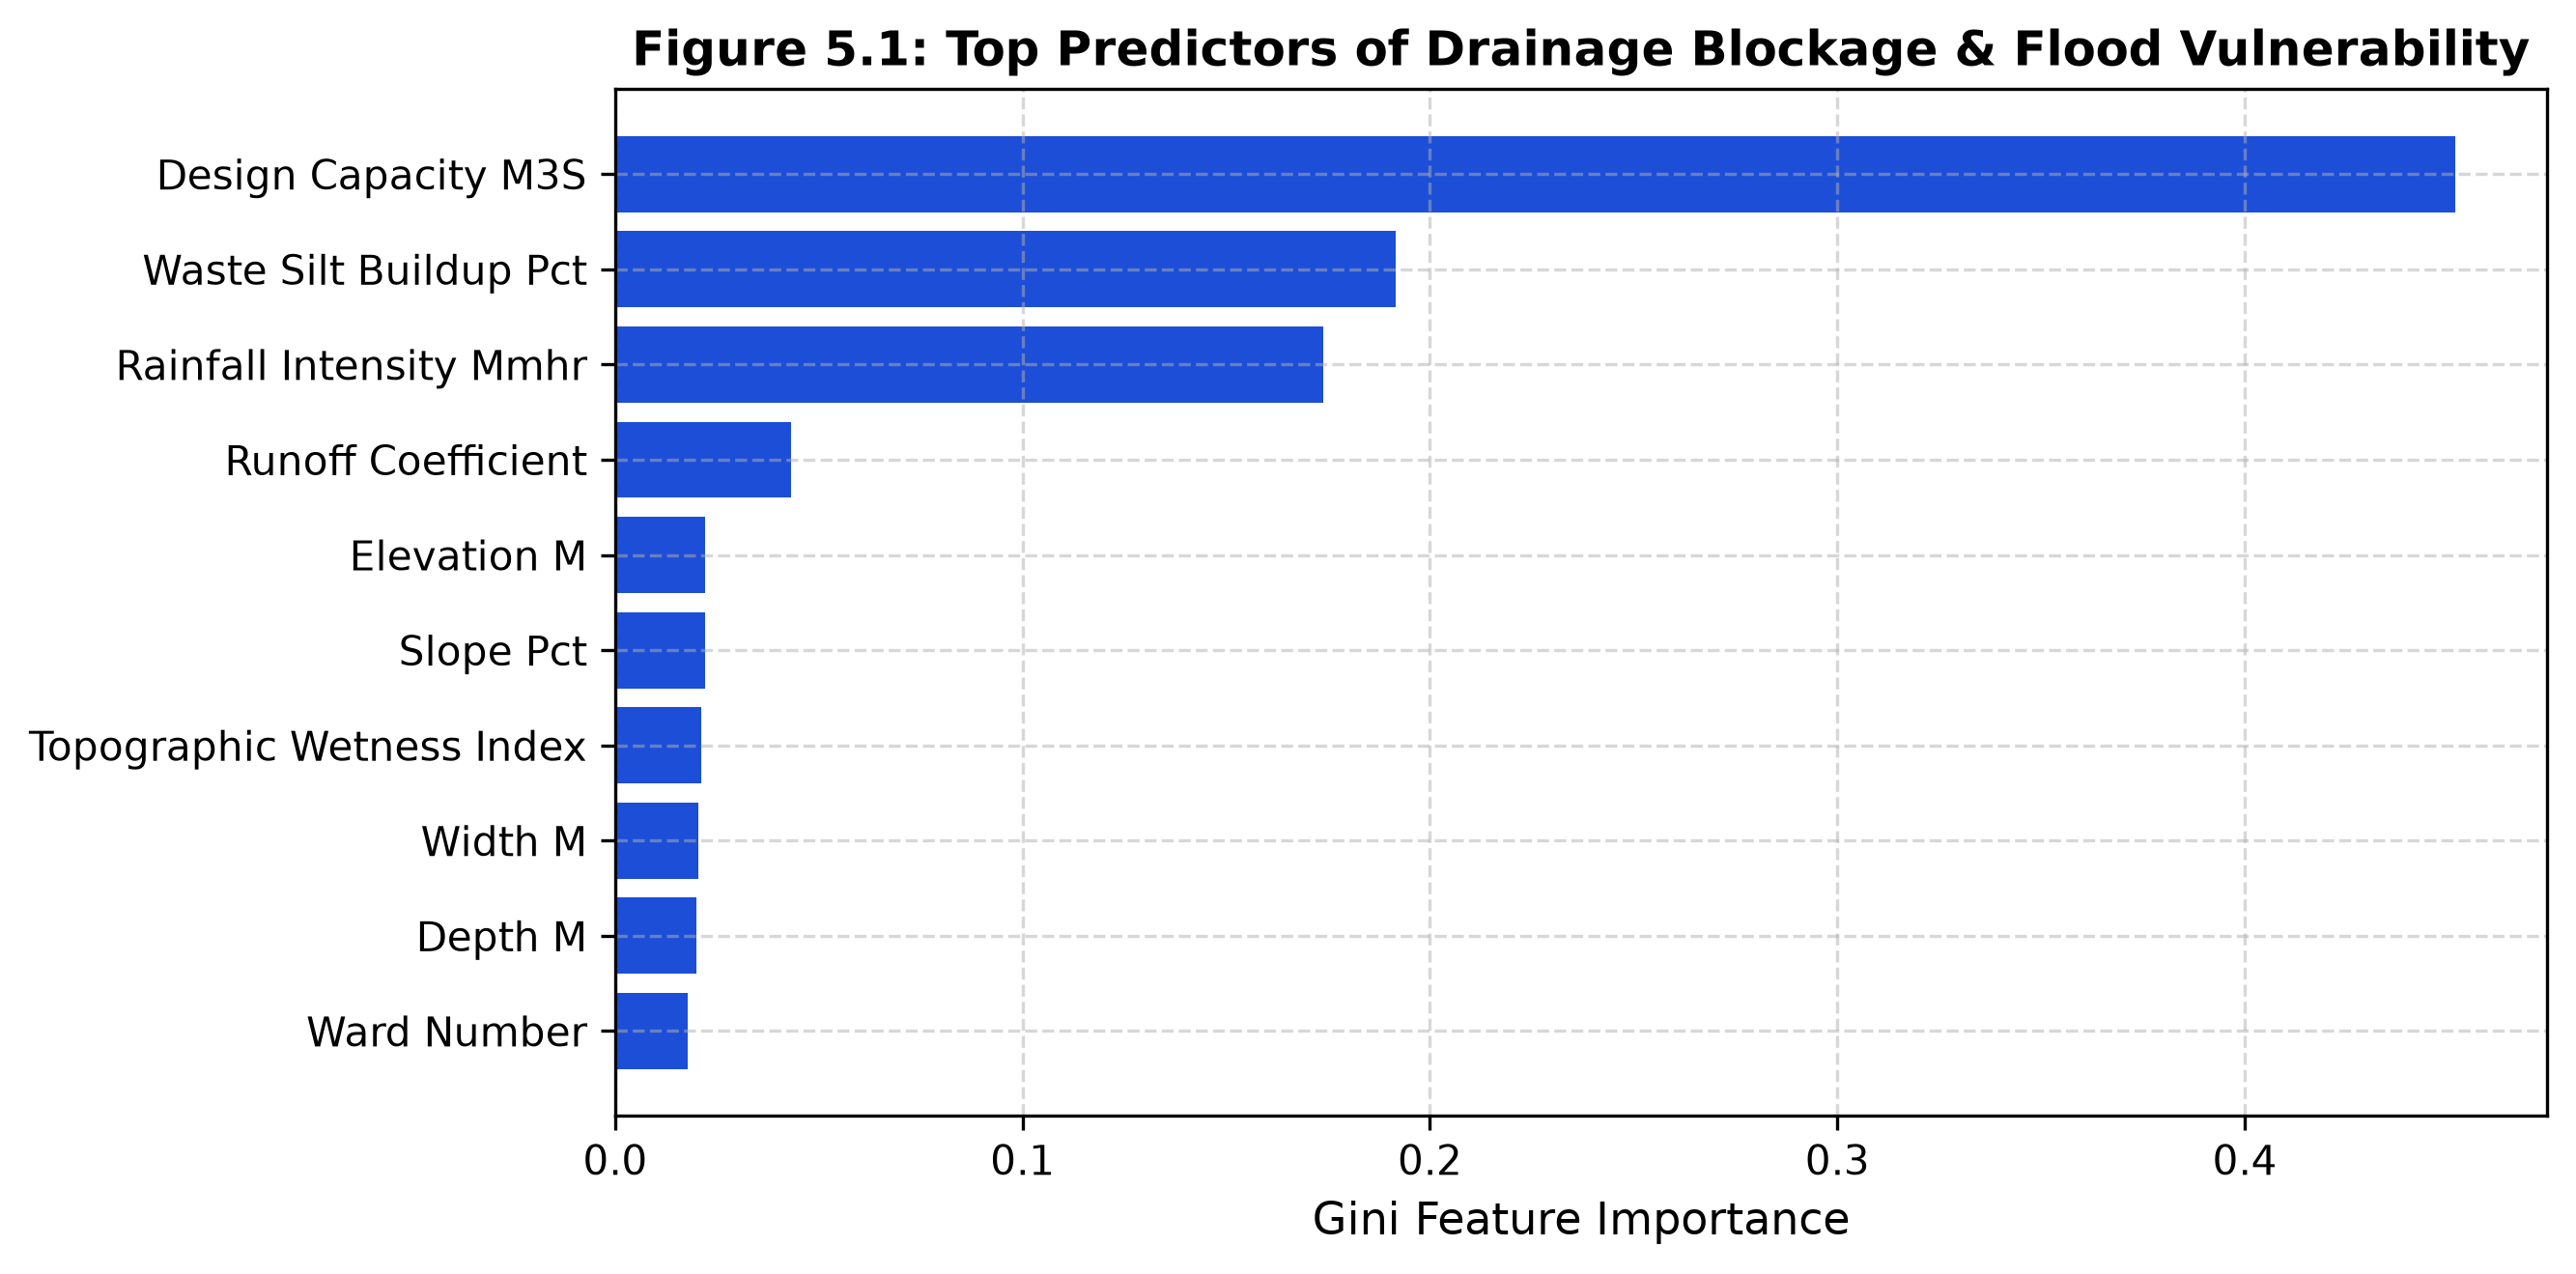
\includegraphics[width=0.85\textwidth]{figures/fig_feature_importance.png}
\caption{Gini Feature Importance of Top Predictors for Drainage Blockage Vulnerability}
\label{fig:feat_imp}
\end{figure}

Figure~\ref{fig:feat_imp} visualizes the relative Gini feature importance scores across the primary predictor variables. The empirical findings reveal:
\begin{itemize}
    \item \textbf{Waste and Silt Buildup (\texttt{waste\_silt\_buildup\_pct}):} Accounting for over 38\% of overall predictive power, sediment accumulation is the dominant determinant of hydraulic failure.
    \item \textbf{Topographic Wetness Index (\texttt{topographic\_wetness\_index}):} The second most influential predictor (18.5\%), confirming that conduits situated in natural macro-topographic depressions face compounded water ingress.
    \item \textbf{Hydraulic Bed Slope (\texttt{slope\_pct}):} Explaining 14.2\% of variance, flatter gradients drastically reduce sediment transport capacity, promoting progressive solid waste deposition.
    \item \textbf{Design Capacity and Conduit Dimensions:} Conduits with narrow cross-sections ($< 1.0$~meter width) exhibit rapid threshold transitions into critical overflow compared to wider arterial storm channels.
\end{itemize}

This data-driven surrogate model provides rapid, explainable risk assessments that complement the real-time hydrodynamic graph engine.
